\documentclass{article}
\usepackage[utf8]{inputenc}
\usepackage[T1]{fontenc}
\usepackage{ngerman}
\usepackage{graphicx}
 
\title{Mustererkennung\\~\\Hausaufgabe 1\\ \small{J. Cavojska, N. Lehmann}}
\date{23.04.2015}


\begin{document}

\maketitle

\section*{Aufgabe 1}

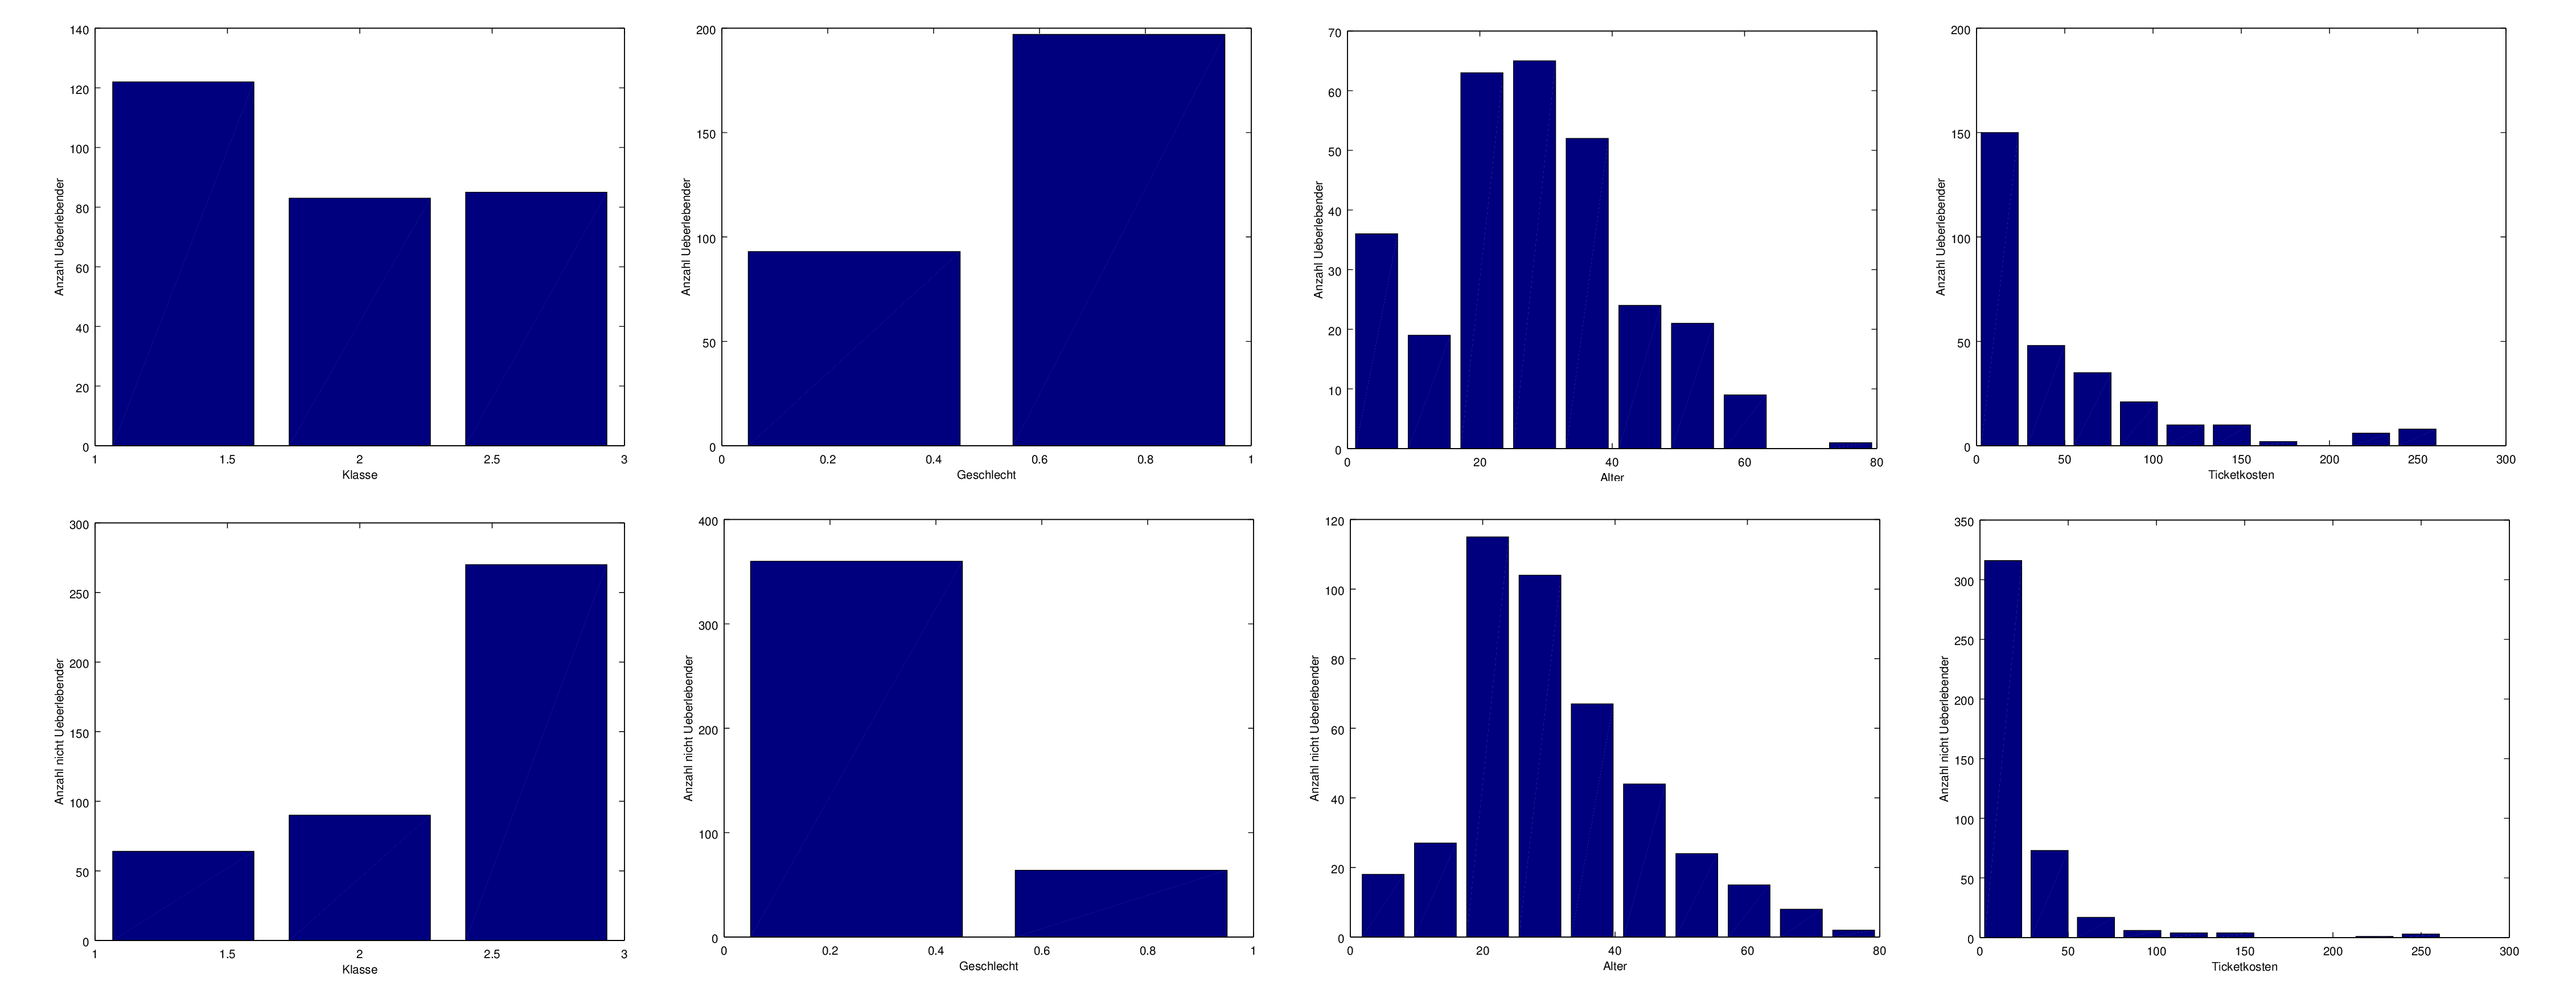
\includegraphics[width=12cm]{Histograms.png}

\begin{verbatim}
A = load('titanic.csv')

% Die Tabelle ueberlebt enthaelt diejenigen Zeilen von Matrix A,
% bei denen die 6. Spalte in Matrix A den Wert 1 (ueberlebt) hat.

nicht_ueberlebt = A(A(:,6)==0,:)
ueberlebt = A(A(:,6)==1,:) 

histogram(ueberlebt(:, 2),3);
xlabel('Klasse');
ylabel('Anzahl Ueberlebender')

histogram(ueberlebt(:, 3),2);
xlabel('Geschlecht');
ylabel('Anzahl Ueberlebender')

histogram(ueberlebt(:, 4));
xlabel('Alter');
ylabel('Anzahl Ueberlebender')

histogram(ueberlebt(:, 5));
xlabel('Ticketkosten');
ylabel('Anzahl Ueberlebender')

histogram(nicht_ueberlebt(:, 2),3);
xlabel('Klasse');
ylabel('Anzahl nicht Ueberlebender')

histogram(nicht_ueberlebt(:, 3),2);
xlabel('Geschlecht');
ylabel('Anzahl nicht Ueberlebender')

histogram(nicht_ueberlebt(:, 4));
xlabel('Alter');
ylabel('Anzahl nicht Ueberlebender')

histogram(nicht_ueberlebt(:, 5));
xlabel('Ticketkosten');
ylabel('Anzahl nicht Ueberlebender')
\end{verbatim}

\section*{Aufgabe 2}

\subsection*{a)}

\begin{verbatim}
% P(U)  = Anzahl der Zeilen von ueberlebt / Anzahl der Zeilen von A:
P_U = size(ueberlebt, 1) / size(A, 1)
% P_U =  0.40616$
\end{verbatim}

\subsection*{b)}

\begin{verbatim}
ueberlebt_maennlich = ueberlebt(ueberlebt(:,3)==0,:)
% P(m|U) = Anzahl der Zeilen von ueberlebt_maennlich / Anzahl der Zeilen von Ueberlebt:
P_m_U = size(ueberlebt_maennlich, 1) / size(ueberlebt, 1)
% P(m|U) =  0.32069
\end{verbatim}

\subsection*{c)}

\begin{verbatim}
maennlich = A(A(:, 3)==0,:)
% P(m)  = Anzahl der Zeilen von maennlich / Anzahl der Zeilen von A:
P_m = size(maennlich, 1) / size(A, 1)
% P(m) =  453 / 714 = 0.63445
\end{verbatim}

\subsection*{d)}

\begin{verbatim}
P(U|m) = P(m|U) * P(U) / P(m) = P_m_U * P_U / P_m
%P(U|m) = 0.20530
\end{verbatim}

\end{document}